\subsection{The Impact of Deviations of the Data from the Idealized qDF} \label{sec:results_mixedDFs}

%Motivation of the test and what we're doing
Our modelling approach assumes that each \MAP follows a quasi-isothermal distribution function, qDF. In this Section we explore what happens if this idealization does not hold. This could be, because even in the limit of perfectly measured abundances, \MAPs do not follow a qDF. Or, even if they do follow a qDF, the finite abundance errors effectively mix different \MAPs. We investigate both these issues by creating mock data sets (Figure \ref{fig:isoSphFlexMix_mockdata_residuals}) that are drawn from two distinct qDFs of different temperature, and analyze the composite mock data set by fitting a single qDF to it. These results are illustrated in Figs. \ref{fig:isoSphFlexMixCont} and \ref{fig:isoSphFlexMixDiff}. Following the observational evidence, \MAPs with cooler qDFs also have longer tracer scale lengths. In the first set of test, we choose qDFs of widely different temperatures and vary their relative fraction (dubbed ``Examples 1a/b" in Figure \ref{fig:isoSphFlexMixCont} and Test \textcircled{7} in Table \ref{tbl:tests}); in the second set of tests (``Examples 2a/b" in Figure \ref{fig:isoSphFlexMixDiff} and Test \textcircled{7} in Table \ref{tbl:tests}), we always mix mock data points from two different qDFs in equal proportion, but vary by how much the qDF's temperatures differ. 
\\The first set of tests mimics a DF that has wider wings or a sharper core in velocity space than a qDF (Figure \ref{fig:isoSphFlexMix_mockdata_residuals}). The second test could be understood as mixing neighbouring \MAPs due to too large bin sizes or abundance measurement errors.

%What we see in the plot
It is worth considering separately the impact of the DF deviations on the recovery of the potential and of the qDF parameters. 
\\We find from Example 1 that the potential parameters can be better and more robustly recovered, if a mock-data \MAP is polluted by a modest fraction ($\lesssim 30\%$) of stars drawn from a much cooler qDF with a longer scale length, as opposed to the same pollution of stars drawn from a hotter qDF with a shorter scale length. 
\\When considering the case of a 50/50 mix of contributions from different qDFs in Example 2, there is a systematic, but only small, error in recovering the potential parameters, monotonically increasing with the qDF parameter difference; in particular for fractional differences in the qDF parameters of $\lesssim 20\%$ the systematics are insignificant even for samples sizes of 20,000, as used in the mock data. 
\\Overall, a cooler DF seems to always give tighter constraints on the circular velocity at the sun $v_\text{circ}(R_\odot)$, because the rotation curve can be constrained easier if more stars are on near-circular orbits. But the recovered $v_\text{circ}(R_\odot)$ does not necessarily have to be right. The hotter DFs give less tight constraints and are therefore more forgiving.
\\The recovery of the effective qDF parameters, in light of non-qDF mock data is quite intuitive: the effective qDF temperature lies between the two temperatures from which the mixed DF of the mock data was drawn; in all cases the scale length of the velocity dispersion fall-off, $h_{\sigma R}$ and $h_{\sigma , z}$, is shorter, because the stars drawn form the hotter qDF dominate at small radii, while stars form the cooler qDF (with its longer tracer scale length) dominate at large radii. The recovered tracer scale lengths, $h_R$ vary smoothly between the input values of the two qDFs that entered the mix of mock data, with again the impact of contamination by a hotter qDF (with its shorter scale length in this case) being more important. 



%====================================================================

%FIGURE: isoSphFlexMix_mockdata_residuals

\begin{figure*}
\plotone{figs/isoSphFlexMix_mockdata_residuals.eps}
\caption{Distribution of mock data, created by mixing stars drawn from two different qDFs (solid lines), and the distribution predicted by the best fit of a single qDF and potential to the data (dashed lines). The model parameters to create the mock data (solid lines) are given in Table \ref{tbl:tests} as Test \textcircled{7}, and the qDF parameters referenced in the figure's legend are given in Table \ref{tbl:referenceMAPs}. The corresponding single qDF best fit curves (dashed lines) were created by drawing mock data from the best fit parameters found in Figures \ref{fig:isoSphFlexMixCont} and \ref{fig:isoSphFlexMixDiff}. \emph{Example 1:} Distribution of mock data drawn from a superposition of two very different (but fixed) qDFs at varying mixing rates. \emph{Example 2:} Mock data distribution of two \MAPs that were mixed at a fixed rate of 50\%/50\%, but the difference of the qDF parameters of one \MAP was varied with respect to the qDF parameters of the other \MAP by $X\%$ (see Table \ref{tbl:referenceMAPs}). The data sets are color coded in the same way as the corresponding analyses in Figures  \ref{fig:isoSphFlexMixCont} and \ref{fig:isoSphFlexMixDiff}. This figure demonstrates how mixing two qDFs can be used as a test case for changing the shape of the DF to not follow a pure qDF anymore, e.g. by adding wings or slightly changing the radial density profile. When comparing the mock data and best fit distribution, we see that especially for the most extreme deviations it becomes obvious that a single qDF is a bad assumption for the stars' "true" DF.}
\label{fig:isoSphFlexMix_mockdata_residuals}
\end{figure*}


%FIGURE: isoSphFlexMixCont

\begin{figure*}
\centering
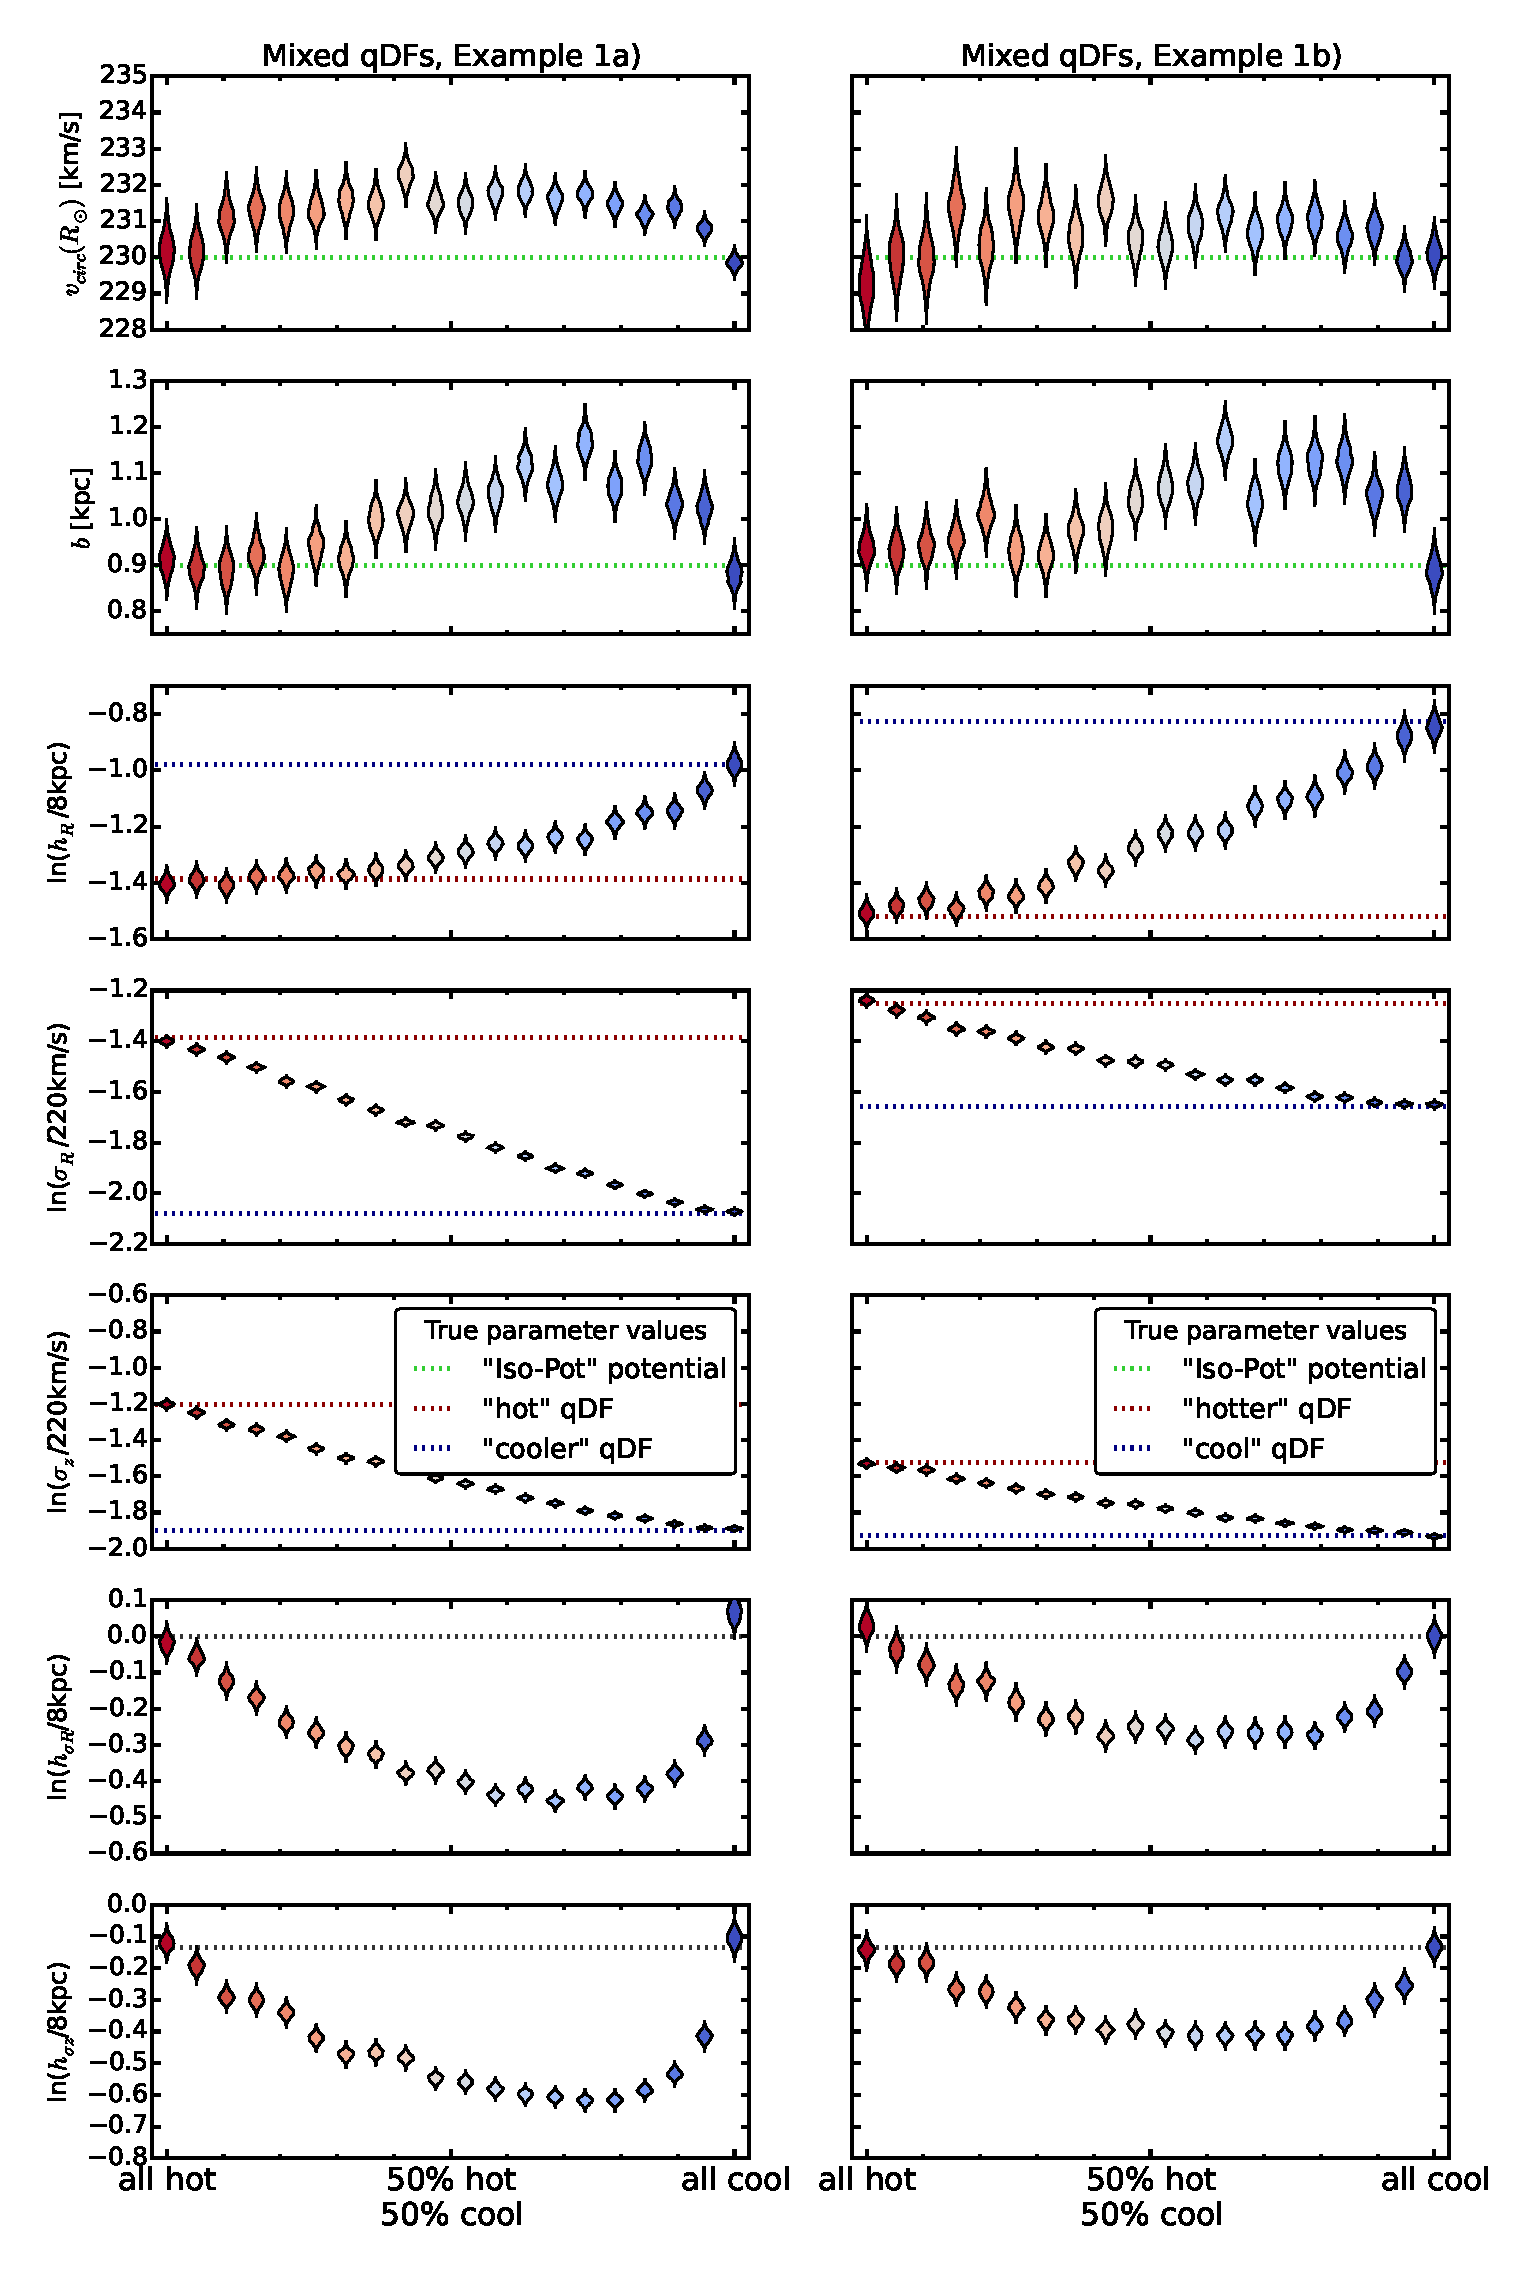
\includegraphics[width=0.8\textwidth]{figs/isoSphFlexMixCont_violins.eps}
\caption{(Caption on next page.)}
\end{figure*}


\addtocounter{figure}{-1}
\begin{figure*} [t!]
\caption{The dependence of the parameter recovery on degree of pollution and temperature of the stellar population. To model the pollution of a hot stellar population by stars coming from a cool population and vice versa, we mix varying amounts of stars from two very different populations, as indicated on the $X$-axis. The composite mock data set is then fit with one single qDF. The violins represent the marginalized likelihoods found from the MCMC analysis. \emph{Example 1a} (\emph{Example 1b}) in the left (right) panels mixes the "hot" ("cool") \MAP with the "cooler" ("hotter") \MAP in Table \ref{tbl:referenceMAPs}. All model parameters used to create the mock data are given in Test \textcircled{7}, \emph{Example 1a) \& b)} in Table \ref{tbl:tests}. Some mock data sets are shown in Figure \ref{fig:isoSphFlexMix_mockdata_residuals}, first two rows, in the same colors as the violins here.  We find, that a hot population is much less affected by pollution with stars from a cooler population than vice versa.}
\label{fig:isoSphFlexMixCont}
\end{figure*}



%FIGURE: isoSphFlexMixDiff

\begin{figure*}
\centering
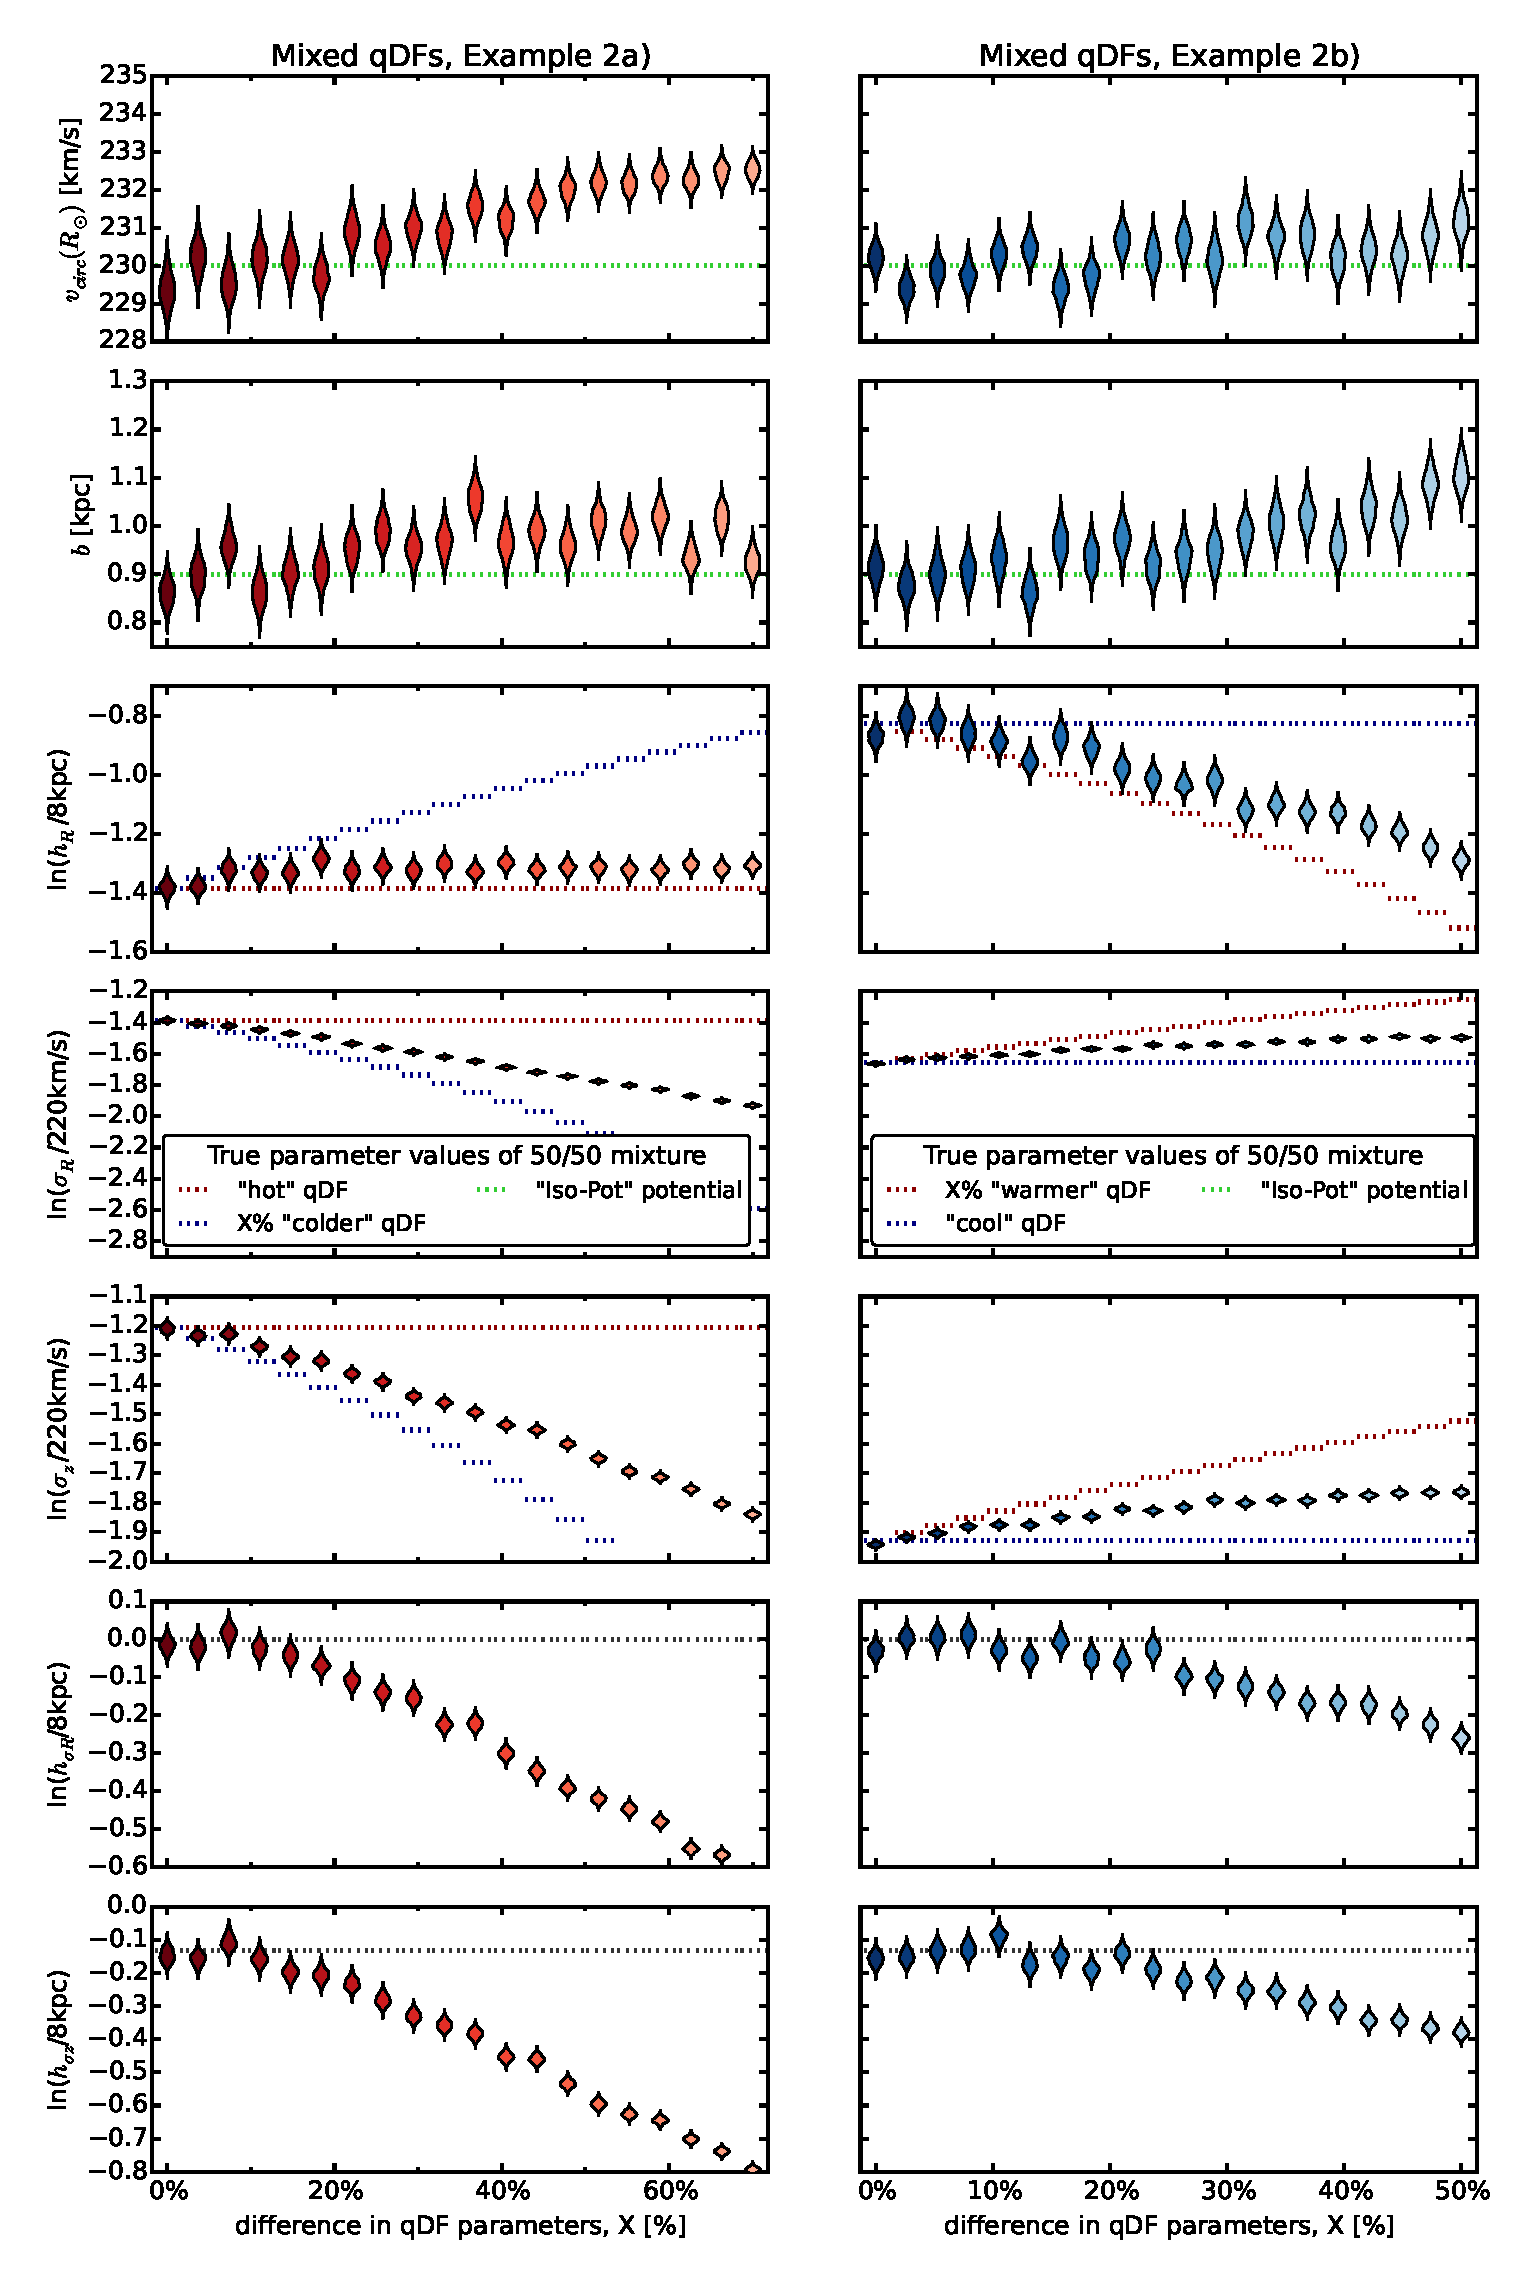
\includegraphics[width=0.8\textwidth]{figs/isoSphFlexMixDiff_violins.eps}
\caption{(Caption on next page.)}
\end{figure*}


\addtocounter{figure}{-1}
\begin{figure*} [t!]
\caption{The dependence of the parameter recovery on the difference in qDF parameters of a 50\%/50\% mixture of two stellar populations and their temperature. Half of the star in each mock data set in \emph{Example 2a} (\emph{Example 2b}) was drawn from the "hot" ("cool") qDF in Table \ref{tbl:referenceMAPs}, and the other half drawn from a "colder" ("warmer") population that has $X\%$ smaller (larger) $\sigma_R$ and $\sigma_z$ and $X\%$ larger (smaller) $h_R$. Each composite mock data set is then fitted by a single qDF and the marginalized MCMC likelihoods for the best fit parameters are shown as violins. The model parameters used for the mock data creation are given as Test \textcircled{7}, \emph{Example 2a) \& b)} in Table \ref{tbl:tests}. Some mock data sets are shown in figure \ref{fig:isoSphFlexMix_mockdata_residuals}, last two rows, where the distributions have the same colors as the corresponding best fit violins here. By mixing \MAPs with varying difference in their qDF parameters, we model the effect of bin size in the [Fe/H]-[$\alpha$/Fe] plane when sorting stars into different \MAPs: The smaller the bin size, the smaller the difference in qDF parameters of stars in the same bin. We find that the bin sizes should be chosen such that the difference in qDF parameters between neighbouring \MAPs is less than 20\%.} 
\label{fig:isoSphFlexMixDiff}
\end{figure*}

%====================================================================
